\documentclass{beamer}
\usepackage{listings}
\lstset{
%language=C,
frame=single, 
breaklines=true,
columns=fullflexible
}
\usepackage{blkarray}
\usepackage{subcaption}
\usepackage{url}
\usepackage{tikz}
\usepackage{tkz-euclide} % loads  TikZ and tkz-base
%\usetkzobj{all}
\usetikzlibrary{calc,math}
\usepackage{float}
\newcommand\norm[1]{\left\lVert#1\right\rVert}
\renewcommand{\vec}[1]{\mathbf{#1}}
\usepackage[export]{adjustbox}
\usepackage[utf8]{inputenc}
\usepackage{amsmath}
\usepackage{amsfonts}
\usepackage{tikz}
\usepackage{hyperref}
\usepackage{bm}
\hypersetup{
    colorlinks = true,
    linkbordercolor = {white},
    linkcolor={red},
    citecolor={green},
    filecolor={blue},
	menucolor={red},
	runcolor={cyan},
	urlcolor={blue},
	breaklinks=true
}
\usetikzlibrary{automata, positioning}
\usetheme{Boadilla}
\providecommand{\pr}[1]{\ensuremath{\Pr\left(#1\right)}}
\providecommand{\mbf}{\mathbf}
\providecommand{\qfunc}[1]{\ensuremath{Q\left(#1\right)}}
\providecommand{\sbrak}[1]{\ensuremath{{}\left[#1\right]}}
\providecommand{\lsbrak}[1]{\ensuremath{{}\left[#1\right.}}
\providecommand{\rsbrak}[1]{\ensuremath{{}\left.#1\right]}}
\providecommand{\brak}[1]{\ensuremath{\left(#1\right)}}
\providecommand{\lbrak}[1]{\ensuremath{\left(#1\right.}}
\providecommand{\rbrak}[1]{\ensuremath{\left.#1\right)}}
\providecommand{\cbrak}[1]{\ensuremath{\left\{#1\right\}}}
\providecommand{\lcbrak}[1]{\ensuremath{\left\{#1\right.}}
\providecommand{\rcbrak}[1]{\ensuremath{\left.#1\right\}}}
\providecommand{\abs}[1]{\vert#1\vert}

\newcounter{saveenumi}
\newcommand{\seti}{\setcounter{saveenumi}{\value{enumi}}}
\newcommand{\conti}{\setcounter{enumi}{\value{saveenumi}}}

\makeatletter
\newenvironment<>{proofs}[1][\proofname]{%
    \par
    \def\insertproofname{#1\@addpunct{.}}%
    \usebeamertemplate{proof begin}#2}
  {\usebeamertemplate{proof end}}
\makeatother

\title{Research Paper Presentation}
\author{Avula Mohana Durga Dinesh Reddy}
\date{CS20BTECH11005}
\begin{document}

\begin{frame}
\titlepage
\end{frame}

\begin{frame}
\frametitle{Title and authors}
\begin{block}{Title}
PROBABILITY REGRESSION SUITES
\end{block}
\begin{block}{Authors}
\begin{enumerate}
\item Shai Fine,fshai@il.ibm.com, IBM Research Laboratory in Haifa ,31905 ,Israel
\item Shmuel Ur, ur@il.ibm.com ,IBM Research Laboratory in Haifa ,31905 ,Israel
\item Avi Ziv ,aziv@il.ibm.com, IBM Research Laboratory in Haifa ,31905 ,Israel
\end{enumerate}
\end{block}
\end{frame}

\begin{frame}{Abstract}
\begin{enumerate}
\item Random test generators are often used to generate regression suites for testing.
\item Regression suites are commonly generated by choosing several specifications and generating a number of tests from each one, without reasoning which specification should be used and how many tests to be generated from each specification.
\item This paper describes about a practical technique for building high quality regression suites, this technique is shown to be cheaper and efficient from experiments.  
\end{enumerate}
\end{frame}

\begin{frame}{Concepts and definitions}
\begin{itemize}
\item \textbf{Regression suite} : It is a set of test specifications.
\item \textbf{Optimisation Problem} : It is the set of dersired conditions the Probabilistic Regression suite is requred to satisfy.
\end{itemize}
\end{frame}

\begin{frame}{Abbreviations}
\begin{center}
\begin{table}[h]
    \centering
    \scalebox{1}{
    \resizebox{\columnwidth}{!}{
\begin{tabular}{|c|c|c|}
\hline
\textbf{Abbreviation} & \textbf{Formula} & \textbf{Meaning} \\
\hline
t & =$\brak{t_1,....t_n}$ &the set of tasks to be covered \\
\hline
s & =$\brak{s_1,....,s_k}$ &the sets of parameters that are allowed to be used in stimulation runs. \\
\hline
$P^i_j$ & &The probability of covering task $t_j$ in a stimulation that uses parameter set\brak{test specification} $s_j$\\
\hline
$w_i$ & $w_i \in \mathbb{N}$ & which denotes the number of times a stimulation, using parameter set $s_i$ must be activated. \\
\hline
policy w & =$\brak{w_1,...,w_k}$ &the activation policy \\
\hline
W & $\sum w_i$ &denotes the total number of stimulation runs derieved by using policy w.\\
\hline
$E_{cnst}$ & & lower bound for expected coverage\\
\hline
$\xi_i$ & $>0$ & additional set of non-negative slack variables for violation magnitude.\\
\hline
$c_i$ & & It is the cost of overall resource consumpltion ehile using the parameter $s_i$\\
\hline
C & & The bound on the total resouce consumption\\
\hline
\end{tabular}
}
}
    \caption{Abbreviations used in presentation}
    \label{Abbreviation table}
\end{table}
\end{center}
\end{frame}

\begin{frame}{Introduction}
\begin{enumerate}
\item Presently, up to 70\% of design development time and resources are spent on functional verification.
\item Current industrial practice uses stimulation-based verification (or dynamic verification) as the main functional verification vehicle for large and complex designs.
\item Regression testing plays an important role in dynamic verification.
\item In Regression testing , a set of tests known as \textit{regression suite} ,is stimulated periodically and after major changes in the design or its environment , in order to check that no bugs were introduced.
\seti 
\end{enumerate}
\end{frame}

\begin{frame}{Introduction Contd.}
\begin{enumerate}
\conti
\item While using a random test generator, test suites don't have to be maintained ,only the generator is maintained for other reasons.As a result , random regression suites are often preferred over maintaining test suites.
\item An important source of information that can be used to create efficient random regression suites is the probability of each test specification to cover each of coverage tasks.Another source can be a Coverage Directed Generation Engine which provides estimates of these probabilities.
\item In this paper we will first show how to construct a regeression suite that uses minimal number of tests required to achieve a specific coverage goal.Then we show how to create a regression suite that maximizes coverage when fixed number of tests are used.
\end{enumerate}
\end{frame}

\begin{frame}{Constructing Probabilistic Regression Suite}
\begin{enumerate}
\item Given a policy w , the probability of covering a task $t_j$ is represented by 
\begin{align}
P_j=E\brak{t_j}&=1-\prod_i \brak{1-P_j^i}^{w_i}
\end{align}
and since the event of covering task $t_j$ is Bernoulli , $P_j = E\brak{t_j}$ is the expected coverage of task $t_j$.
\seti
\item Firstly lets define \textit{optimisation problem} as :\textbf{Probabilistic Regression Suite}. \textit{Find the policy w , which minimises the number of stimulation runs and with high probability provides a desired coverage.}
\begin{align}
min_w &\hspace{10pt} \sum w_i \nonumber \\
\text{such that }\forall j &\hspace{10pt}  P_j = 1- \prod_i \brak{1-P^i_j}^{w_i} \geq E_{cnst} \nonumber \\
\forall i &\hspace{10pt}  \mathbb{N} \ni w_i \geq 0 
\end{align}
\end{enumerate}
\end{frame}

\begin{frame}{Constructing Probabilistic Regression Suite Contd.}
\begin{enumerate}
\conti
\item This is a integer programming\brak{IP} problem which is difficult to solve. So we use a relaxation technique by applying log.The resulting \textit{optimisation problem} is linear.
\begin{align}
min_w &\hspace{10pt} \sum w_i \nonumber \\
\text{such that }\forall j &\hspace{10pt} \sum_i w_i \times g_{ij}\leq log\brak{1- E_{cnst}} \nonumber \\
\forall i &\hspace{10pt}  \mathbb{N} \ni w_i \geq 0 
\end{align}
where $g_{ij} = log\brak{1-E_{cnst}}$\\
\seti
\item Now lets focus on the tasks that have too small probabilities, the number of stimulation runs required to cover these tasks is too high so we will instead "charge" the objective function with violation magnitude times cost c , for each violation constraint.
\end{enumerate}
\end{frame}

\begin{frame}{Constructing Probabilistic Regression Suite Contd.}
\begin{enumerate}
\conti
\item Lets add this property to the optimisation problem.\\
The definition of \textit{Optimisation problem} becomes :\textbf{Soft Probabilistic Regression Suite}. \textit{Find the policy w , which minimises the number of stimulation runs and with high probability provides a coverage that permits violation of the lower bounds for task coverage.}
\begin{align}
min_w &\hspace{10pt} \sum w_i +c\sum_i \xi_i \nonumber \\
\text{such that }\forall j &\hspace{10pt} \sum_i w_i \times g_{ij}\leq log\brak{1- E_{cnst}} \nonumber \\
\forall i &\hspace{10pt}  \mathbb{N} \ni w_i \geq 0 \nonumber \\
\forall j &\hspace{10pt} \xi_i \geq 0
\end{align}
\seti
\end{enumerate}
\end{frame}

\begin{frame}{Constructing Probabilistic Regression Suite Contd.}
\begin{enumerate}
\item Now lets add another property to optimisation problem which is slightly different yet very common scenario of \textit{limited number of resources}.\\
The definition of \textit{Optimisation problem} becomes :\textbf{Expected Coverage Probability with}. \textit{Given a bound on the number of stimulations permitted, W, and a bound on the cost of the resource consumption C, find the policy w, which maximises the expected coverage probability} 
\begin{align}
max_w & \hspace{10pt} \sum_j \brak{1-\prod_i\brak{1-P^i_j}^{w_i}} \nonumber \\
\text{such that} &\hspace{10pt} \sum_i w_i \leq W \nonumber \\
&\hspace{10pt} \sum_i c_i w_i \leq C \nonumber \\
\forall i &\hspace{10pt} w_i\geq 0
\end{align}
\seti
\end{enumerate}
\end{frame}

\begin{frame}{Constructing Probabilistic Regression Suite Contd.}
\begin{enumerate}
\conti
\item In the next step we focus on covering the least probable tasks to cover.So the definition of \textit{Optimisation problem } becomes : \textbf{Least Probable Coverage Task with Limited Resources}. \textit{Given a bound on the total number of stimulations W, and a bound on the cost of resource consumption C,find the policy w that maximizes the probability of the least probable task to cover}
\begin{align}
max_w & \hspace{10pt} min_j \brak{1-\prod_i\brak{1-P^i_j}^{w_i}} \nonumber \\
\text{such that} &\hspace{10pt}  w_i \leq W \nonumber \\
&\hspace{10pt} \sum_i c_i w_i \leq C \nonumber \\
\forall i &\hspace{10pt} w_i\geq 0
\end{align}
\end{enumerate}
\end{frame}

\begin{frame}{Experimiental Results}
\begin{figure}[ht]
    \centering
    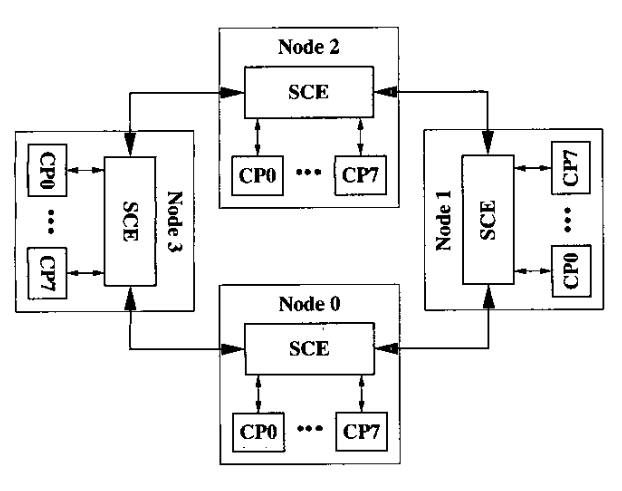
\includegraphics[width=0.5\textwidth]{figures/node.png}
    \caption{Structure of the SCE stimulation environment of an IBM z-series system}
    \label{SCE model}
\end{figure}
\end{frame}

\begin{frame}{Regression suite for Hardware Verification with minimal Number of Stimulations}
\begin{enumerate}
\item Many experiments were conducted of a coverage model used in the verification of the Storage Control Element \brak{SCE} of an IBM z-series as shown in Figure 1.
\item It contains six attributes : the core that initiated the command, the pipeline in the SCE that handled it , the command itself, and three attributes that relate to the response.
\item In the first experiment ,we concentrated on a subset of the coverage model that deals with unrecoverable errors\brak{UE}.The size of UE is 98 all of ehich are hard to cover.
\seti 
\end{enumerate}
\end{frame}

\begin{frame}{Regression suite for Hardware Verification with minimal Number of Stimulations Contd.}
\begin{figure}[ht]
    \centering
    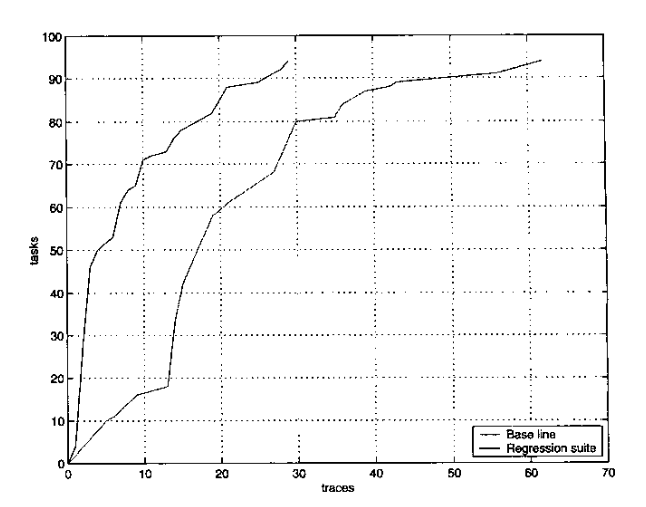
\includegraphics[width=0.5\textwidth]{figures/coverage process ue.png}
    \caption{Coverage process of UE subset of the SCE}
    \label{UE coverage}
\end{figure}
\end{frame}

\begin{frame}{Regression suite for Hardware Verification with minimal Number of Stimulations Contd.}
\begin{figure}[ht]
    \centering
    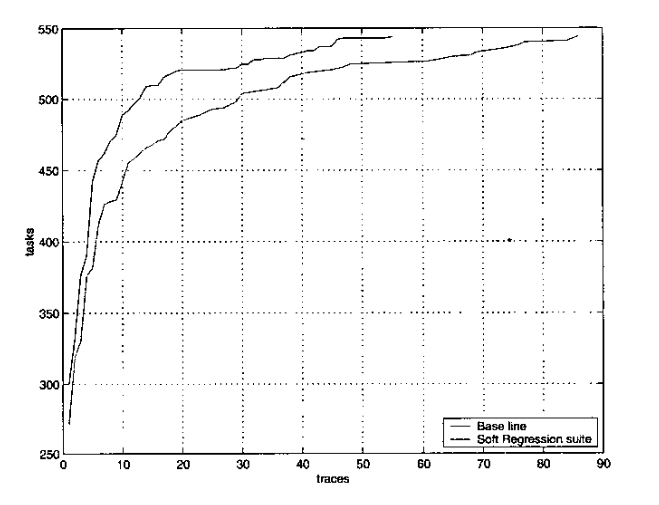
\includegraphics[width=0.5\textwidth]{figures/coverage process sce.png}
    \caption{Coverage process of SCE model}
    \label{SCE coverage}
\end{figure}
\end{frame}

\begin{frame}{Regression suite for Hardware Verification with minimal Number of Stimulations Contd.}
\begin{enumerate}
\conti
\item Using definition Probabilistic Regression Suite with a lower bound of 1/2 for expected coverage it took only 29 stimulations to cover 94 events \brak{96\%}. This when compared to Common practice toom 61 stimulations to cover the same coverage as shown in  \ref{UE coverage}. 
\item The second experiment tageted the whole SCE coverage model which has 564 tasks, most of which aren't hard to cover . The repository we used had 126 test specifications.\\
In this experiment we used definition \textbf{Soft Probabilistic Regression suite} with a lower bound of 1/2 for expected coverage. It took only 55 stimulations to cover 554 events \brak{98\%}. This when compared to activation of every parameter set one by one , it took 86 stimulations to reach same coverage as shown in \ref{SCE coverage}.
\end{enumerate}
\end{frame}

\begin{frame}
\begin{figure}[ht]
    \centering
    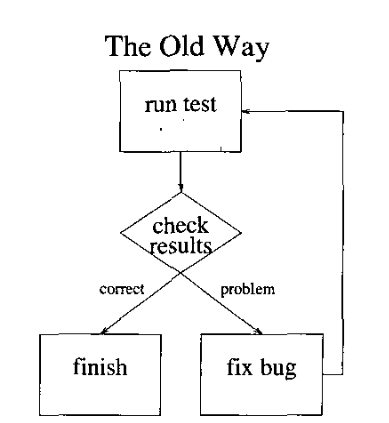
\includegraphics[width=0.5\textwidth]{figures/old way testing.png}
    \caption{Each test executed once}
    \label{old way}
\end{figure}
\end{frame}

\begin{frame}
\begin{figure}[ht]
    \centering
    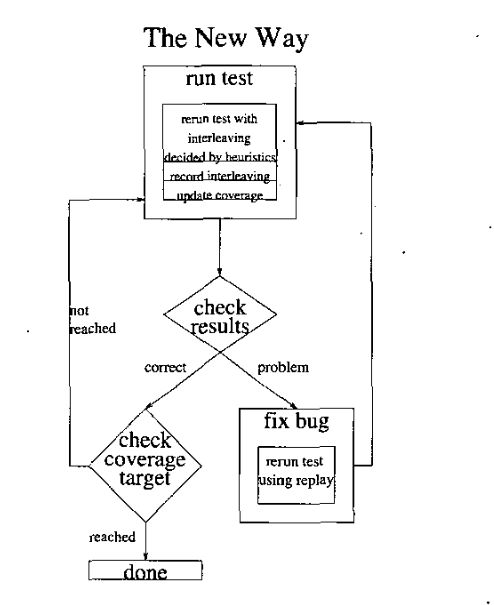
\includegraphics[width=0.5\textwidth]{figures/new way testing.png}
    \caption{Executiong until reaching coverage target}
    \label{new way}
\end{figure}
\end{frame}

\begin{frame}{Regression suite for Software Testing with a limited Number of Test Executions}
\begin{enumerate}
\item A test in the multi-threaded domain is a combination of inputs and interleaving , where interleaving is the relative order in which the threads were executed. Running the same inputs twice may result in different outcomes. 
\item The process depicted in \ref{old way} Load testing (i.e testing the applicatication under a real or stimulated workload), increases the likelihood of some interleaving that would be unlikely under light load. However , load testing is not systematic and is expensive and can be only executed at the end of the testing cycle.
\item ConTest is a tool fo rgenerating different interleaving for the purpose of revealing concurrent faults.ConTest takes a heuristic approach of seeding the program with instrumentation in concurrently significant locations.  
\item The process of re-execcuting tests using ConTest is depicted in \ref{new way} . Each time the functional test t is run as a result od seding technique , ConTest produces a potentially different interleaving.
\seti
\end{enumerate}
\end{frame}

\begin{frame}{Regression suite for Software Testing with a limited Number of Test Executions Contd.}
\begin{enumerate}
\conti
\item For the experiment we used 13 different heuristics as the test apecifications.Given the statistics collected for the 13 heuristics we constructed policies designed to maximize the coverage of the 10,000 events using no more than 250 and 1000 test runs.We used definition \textbf{Expected Coverage with limited probability} while using greedy technique to  get the solutions.
\item The policy was designed to yield best coverage with 250 runs using only 2 heuristics.The policy for the 1000 runs was constructed on 4 heuristcs, two of which are dominant(used roughly 83\% of the time) 
\seti
\end{enumerate}
\end{frame}

\begin{frame}{Regression suite for Software Testing with a limited Number of Test Executions Contd.}

\begin{center}
\begin{table}[ht]
    \centering
    \scalebox{0.5}{
    \resizebox{\columnwidth}{!}{
\begin{tabular}{|c|c|c|}
\hline
 & \multicolumn{2}{|c|}{Num. Events Covered} \\
\hline
 & 250 &1000 \\
\hline
Uniform Policy & 1449 & 1988\\
\hline
Best Pure Heuristic & 1699 & 2258 \\
\hline 
Greedy Policy & 1723 & 2429 \\
\hline
\end{tabular}
}
}
    \caption{Total coverage using ConTest for 250 and 1000 test runs}
    \label{Result table}
\end{table}
\end{center}
The first row shows the result averaged over all policies.Second row shows the result of the best policy.Third row shows the result generated by greedy policy.
\begin{enumerate}
\conti
\item table \ref{Result table} shows the number of events covred using 250 ,1000 test runs. Note in passing every heuristic in the 1000 test runs and combinig the results (i.e a total of 13,000 test runs) , only 4338 events were covered . 
\end{enumerate}
\end{frame}

\begin{frame}{Conclusions and Future work}
\begin{enumerate}
\item We have sown that regression suites created are better than those generated at random.This is true for both limited resource and specific utilities scenarios.
\item Experiments shows that our technique is economically rewarding.
\item First we plan to investigate the use of the proposed technique to guide the entire functional verification process.
\item We also investigate the use of hybrid schemes that combines the building of probabilistic regression suites with snapshots of current coverage.
\item Special  attention should be given to tasks that are coveraged with a very low probabilty.One possible solution to this issue is try not to cover these tasks using a random regression suite.Instead, keep tests that cover such tasks along with other tests that are kept in a deterministic regression suite.
\end{enumerate}
\end{frame}

\end{document}